\chapter{Estimaci\'{o}n de la profundidad}
\label{chap:profundidad}
\epigraph{The most powerful source of human depth perception is stereopsis, the response created in our visual systems by comparing the views we get from our two eyes.}{Barry Hochfelder}

En este cap\'{i}tulo se describe el proceso utilizado para la recuperaci\'{o}n de la profundidad de los puntos del objeto. El m\'{e}todo utilizado popularmente es triangulaci\'{o}n. Para la t\'{e}cnica se utiliz\'{o} uno de los algoritmos propuestos por \cite{hartley1997triangulation}. Cabe destacar la importancia en la selecci\'{o}n del algoritmo de triangulaci\'{o}n dado su papel en la calidad de la representaci\'{o}n tridimensional que se obtenga.

\section{Triangulaci\'{o}n}
Recobrar la dimensi\'{o}n perdida (profundidad) de un punto que aparece en un par de im\'{a}genes bidimensionales estereosc\'{o}picas es uno de los problemas m\'{a}s desafiantes en el \'{a}rea de la visi\'{o}n artificial. Para estimar la estructura tridimensional del objeto se deben utilizar las matrices de la c\'{a}mara \textit{P} y \textit{P'} en conjunto con un algoritmo robusto de triangulaci\'{o}n. %Se asume que solamente existen errores en la medici\'{o}n de las coordenadas de la imagen y no en las matrices \textit{P}, \textit{P'}.

De acuerdo con \cite{hartley1997triangulation}, triangulaci\'{o}n se define como el problema de encontrar la posici\'{o}n de un punto en el espacio tridimensional dada su posici\'{o}n en dos im\'{a}genes tomadas con c\'{a}maras de las cuales son conocidos sus valores de calibraci\'{o}n y su posici\'{o}n. Este proceso, requiere la intersecci\'{o}n de dos rayos conocidos en el espacio. En la figura ~\ref{fig:IdealTriangulation} se muestra el caso ideal del proceso de triangulaci\'{o}n.

\begin{figure}[H]
\centering
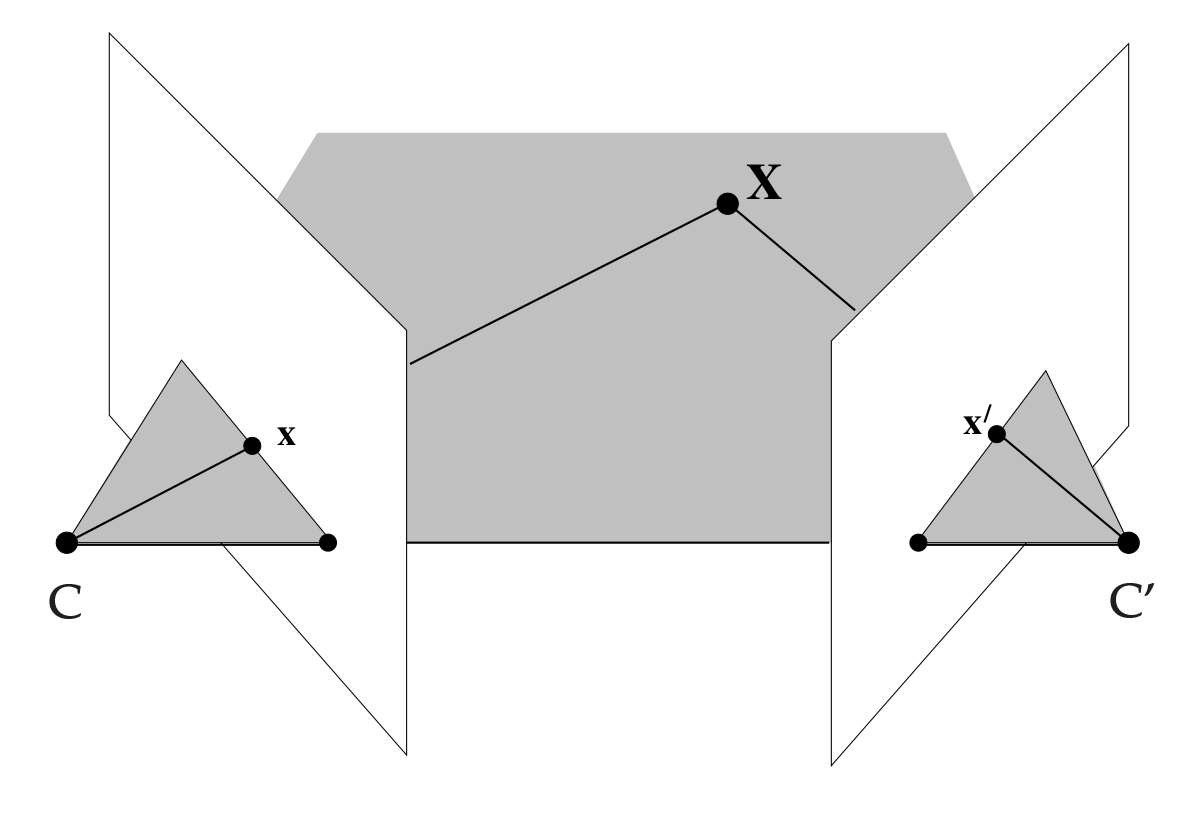
\includegraphics[width=0.8\textwidth]{images/idealtriangulation.png}
\caption[Caso ideal del proceso de triangulaci\'{o}n]%
{Caso ideal de geometr\'{i}a epipolar. Un punto tridimensional \textit{\textbf{X}} es proyectado en dos c\'{a}maras por medio de las l\'{i}neas las cuales se intersecan con el punto focal de cada c\'{a}mara \textbf{\textit{$C$}} y \textbf{\textit{$C'$}}. Los puntos de la imagen resultante son \textbf{\textit{$x$}} y \textbf{\textit{$x'$}}. Las l\'{i}neas se intersecan en \textit{\textbf{X}}. Imagen tomada del libro \textit{Multiple View Geometry} de Richard Hartley y Andrew Zisserman \copyright.}
\label{fig:IdealTriangulation}
\end{figure}

En ausencia de ruido, el problema es trivial. Dado que cada punto en una imagen corresponde a una l\'{i}nea en el espacio tridimensional, todos los puntos de la l\'{i}nea son proyectados en el punto de la imagen. Si es posible encontrar un par de puntos que corresponden en dos o m\'{a}s im\'{a}genes, debe ser el caso en el cual son la proyecci\'{o}n de un punto tridimensional com\'{u}n \textbf{\textit{x}}. El grupo de l\'{i}neas generadas por los puntos de la imagen deben intersecar en \textit{x} y la f\'{o}rmula algebraica para determinar las coordenadas de \textit{x} puede ser calculada utilizando alguno de los muchos m\'{e}todos existentes \cite{hartley1997triangulation,Hartley_Zisserman_2003,Faugeras_1993}.

En la pr\'{a}ctica nada de esto funciona debido la enorme cantidad de ruido (ruido geom\'{e}trico, distorsi\'{o}n del lente, error en los pareos, entre otros) que existe. Esto causa que los dos rayos generalmente no se intersecten por lo que es necesario encontrar el \textit{mejor} punto de la intersecci\'{o}n. En la figura ~\ref{fig:RealTriangulation} se muestra el caso real del proceso de triangulaci\'{o}n.


\begin{figure}[H]
\centering
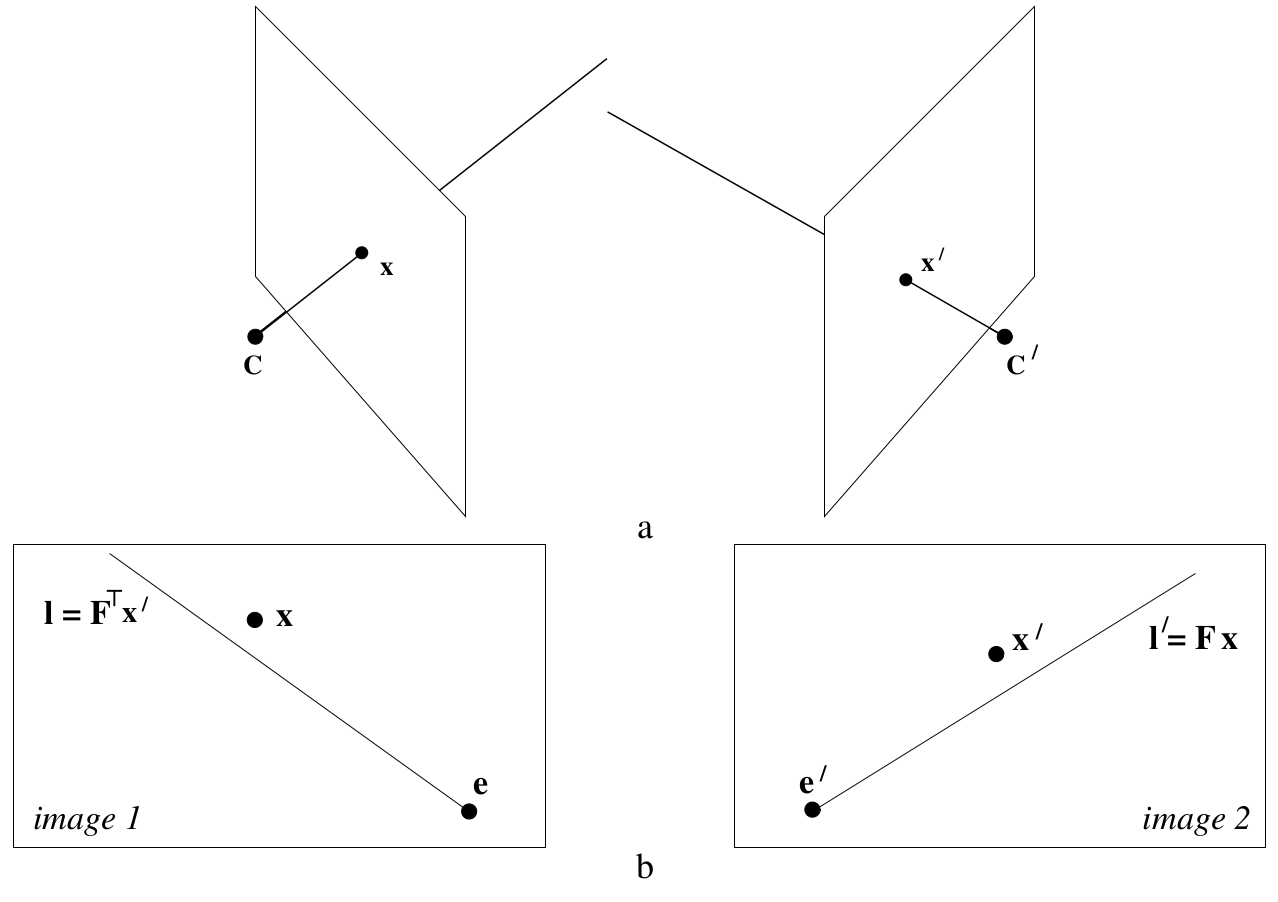
\includegraphics[width=1.0\textwidth]{images/realtriangulation.png}
\caption[Caso real del proceso de triangulaci\'{o}n]%
{En la pr\'{a}ctica, los puntos \textbf{\textit{$x$}} y \textbf{\textit{$x'$}} de la imagen no pueden ser calculados con precisi\'{o}n arbitraria. \textbf{(a)} Los rayos retroproyectados a partir de medidas imperfectas en los puntos \textit{x} y \textit{x'} son generalmente oblicuos en el espacio tridimensional. \textit{(b)} La geometr\'{i}a epipolar para \textbf{\textit{$x$}} y \textbf{\textit{$x'$}}. Los puntos medidos no satisfacen la restricci\'{o}n epipolar. La l\'{i}nea epipolar $l' = Fx$ es la imagen del rayo a trav\'{e}s de \textit{x} y $l = F^Tx'$ es la imagen del rayo a trav\'{e}s de \textit{x'}. Dado que los rayos no se intersecan, \textit{x'} no se encuentra en \textit{l'} y \textit{x} no se encuentra en \textit{l}. Imagen tomada del libro \textit{Multiple View Geometry} de Richard Hartley y Andrew Zisserman \copyright.}
\label{fig:RealTriangulation}
\end{figure}


La importancia en la selecci\'{o}n de un buen algoritmo de triangulaci\'{o}n se muestra claramente en \cite{Beardsley_Zisserman_Murray_1997,beardsley_etal_eccv1994}. En \cite{hartley1997triangulation} se presenta una detallada comparaci\'{o}n entre diferentes algoritmos de triangulaci\'{o}n. En su apartado de resultados se muestra la duraci\'{o}n relativa en tiempo de cada algoritmo as\'{i} como las condiciones bajo las cuales es recomendable utilizar uno en favor del otro. 

Para la t\'{e}cnica de reconstrucci\'{o}n propuesta, se opt\'{o} por utilizar el algoritmo iterativo de m\'{i}nimos cuadrados (del ingl\'{e}s \textit{iterative linear least squares}) descrito en \cite{hartley1997triangulation,Hartley_Zisserman_2003}, dado que seg\'{u}n los resultados de rendimiento mostrados en el art\'{i}culo, es uno de los m\'{a}s r\'{a}pidos (3 veces m\'{a}s que el algoritmo polinomial recomendado por los autores del art\'{i}culo) y desempe\~na bien en reconstrucci\'{o}n tridimensional.

El siguiente paso en la t\'{e}cnica es utilizar las matrices de la c\'{a}mara, el algoritmo de triangulaci\'{o}n y los pareos de puntos clave de la primera fase, para determinar la posici\'{o}n en el espacio tridimensional de cada uno de ellos y as\'{i} reconstruir el objeto en cuesti\'{o}n.

%@TODO resumen del capitulo

%Su \'{u}nico problema es que en ciertos casos no converge y por lo tanto se debe contar con un algoritmo de respaldo.

%@TODO poner screenshots de ejemplos de triangulaci\'{o}n ???
%@TODO es necesario explicar el algoritmo de minimos cuadrados o no???

%\section{Algoritmo iterativo de m\'{i}nimos cuadrados}

%Once we have two camera matrices, P and P', we can recover the 3D structure of the scene. This can be seen simply if we think about it using ray intersection. We have two points in space of the camera centers (one in 0,0,0 and one in t), and we have the location in space of a point both on the image plane of image 1 and on the image plane of image 2. If we simply shoot a ray from from one camera center through the respective point and another ray from the other camera - the intersection of the two rays must be the real location of the object in space.
%In real life, none of that works. The rays usually will not intersect (so H&Z refer to the mid-point algorithm, which they dismiss as a bad choice), and ray intersection in general is inferior to other triangulation methods.
%H&Z go on to describe their "optimal" triangulation method, which optimizes the solution based on the error from reprojection of the points back to the image plane.
%I have implemented the linear triangulation methods they present, and wrote a post about it not long ago: Here.
%I also added the Iterative Least Squares method that Hartley presented in his article "Triangulation", which is said to perform very good and very fast.

